%% Font size %%
\documentclass[11pt]{article}

%% Load the custom package
\usepackage{Mathdoc}

%% Numéro de séquence %% Titre de la séquence %%
\renewcommand{\centerhead}{}

%% Spacing commands %%
\renewcommand{\baselinestretch}{1}
\setlength{\parindent}{0pt}

\begin{document}

% @see : https://coopmaths.fr/alea?uuid=0d1f7&id=3G30-1&n=2&d=10&s=3&s2=4&alea=u9Lf&cd=1&cols=2
\begin{exercice}{}{3G30-1}


\begin{enumerate}[itemsep=2em]
	\item \begin{minipage}[t]{\linewidth} \begin{minipage}{.4\linewidth}
\begin{tikzpicture}[baseline,scale = 0.5]

    \tikzset{
      point/.style={
        thick,
        draw,
        cross out,
        inner sep=0pt,
        minimum width=5pt,
        minimum height=5pt,
      },
    }
    \clip (-7.618630029195217,-6.673111453595901) rectangle (2.95340892674294,1);
    	\draw[color={black}] (0,0)--(-6.62,-2.28)--(1.95,-5.67)--cycle;
	\draw[color={black}] (-0.38,-0.13)--(-0.25,-0.51)--(0.13,-0.38);
	
	\draw [color={black}] (0.25,0.43) node[anchor = center,scale=1, rotate = 0] {T};
	\draw [color={black}] (-7.12,-2.24) node[anchor = center,scale=1, rotate = 0] {V};
	\draw [color={black}] (2.33,-6) node[anchor = center,scale=1, rotate = 0] {S};
	\draw[color ={black}] (0,0)--(-1.6771016898896913,-4.235595719404737);
	\draw [color={black}] (-1.86,-4.7) node[anchor = center,scale=true, rotate = -1] {$U$};
	\draw[color={black}] (-1.53,-3.86)--(-1.9,-3.72)--(-2.05,-4.09);

\end{tikzpicture}\\\\
\end{minipage}
\begin{minipage}{.6\linewidth}
Exprimer $\tan(\widehat{TVS})$ de deux manières différentes.\\Parmi deux triangles, dans le triangle rectangle le plus grand, $\tan\left(\widehat{TVS}\right)=$ $\ldots$\\Parmi deux triangles, dans le triangle rectangle le plus petit, $\tan\left(\widehat{TVS}\right)=$ $\ldots$\\Exprimer $\sin(\widehat{TVS})$ de deux manières différentes.\\Parmi deux triangles, dans le triangle rectangle le plus grand, $\sin\left(\widehat{TVS}\right)=$ $\ldots$\\Parmi deux triangles, dans le triangle rectangle le plus petit, $\sin\left(\widehat{TVS}\right)=$ $\ldots$\\Exprimer $\cos(\widehat{TVS})$ de deux manières différentes.\\Parmi deux triangles, dans le triangle rectangle le plus grand, $\cos\left(\widehat{TVS}\right)=$ $\ldots$\\Parmi deux triangles, dans le triangle rectangle le plus petit, $\cos\left(\widehat{TVS}\right)=$ $\ldots$\\
\end{minipage}
 \end{minipage}
	\item \begin{minipage}[t]{\linewidth} \begin{minipage}{.4\linewidth}
\begin{tikzpicture}[baseline,scale = 0.5]

    \tikzset{
      point/.style={
        thick,
        draw,
        cross out,
        inner sep=0pt,
        minimum width=5pt,
        minimum height=5pt,
      },
    }
    \clip (-7.913818384165964,-6.926130043570827) rectangle (1.938606790241384,1);
    	\draw[color={black}] (0,0)--(-6.91,-1.1)--(0.94,-5.93)--cycle;
	\draw[color={black}] (-0.4,-0.06)--(-0.33,-0.46)--(0.06,-0.4);
	
	\draw [color={black}] (0.32,0.38) node[anchor = center,scale=1, rotate = 0] {I};
	\draw [color={black}] (-7.4,-0.97) node[anchor = center,scale=1, rotate = 0] {H};
	\draw [color={black}] (1.26,-6.31) node[anchor = center,scale=1, rotate = 0] {F};
	\draw[color ={black}] (0,0)--(-2.3871262248017273,-3.8800218508836313);
	\draw [color={black}] (-2.65,-4.31) node[anchor = center,scale=true, rotate = -1] {$G$};
	\draw[color={black}] (-2.18,-3.54)--(-2.52,-3.33)--(-2.73,-3.67);

\end{tikzpicture}\\\\
\end{minipage}
\begin{minipage}{.6\linewidth}
Exprimer $\tan(\widehat{IHF})$ de deux manières différentes.\\Parmi deux triangles, dans le triangle rectangle le plus grand, $\tan\left(\widehat{IHF}\right)=$ $\ldots$\\Parmi deux triangles, dans le triangle rectangle le plus petit, $\tan\left(\widehat{IHF}\right)=$ $\ldots$\\Exprimer $\sin(\widehat{IHF})$ de deux manières différentes.\\Parmi deux triangles, dans le triangle rectangle le plus grand, $\sin\left(\widehat{IHF}\right)=$ $\ldots$\\Parmi deux triangles, dans le triangle rectangle le plus petit, $\sin\left(\widehat{IHF}\right)=$ $\ldots$\\Exprimer $\cos(\widehat{IHF})$ de deux manières différentes.\\Parmi deux triangles, dans le triangle rectangle le plus grand, $\cos\left(\widehat{IHF}\right)=$ $\ldots$\\Parmi deux triangles, dans le triangle rectangle le plus petit, $\cos\left(\widehat{IHF}\right)=$ $\ldots$\\
\end{minipage}
 \end{minipage}
\end{enumerate}

\end{exercice}

% @see : https://coopmaths.fr/alea?uuid=f13e3&id=3G30-2&n=6&d=10&s=3&alea=mt0A&cd=1&cols=2
\begin{exercice}{}{3G30-2}


\begin{enumerate}[itemsep=1em]
	\item \begin{minipage}[t]{\linewidth} Dans le triangle rectangle $GHI$, on a : $\sin\left( 43 ^\circ \right) = \dfrac{5,9}{GI}$.\\Calculer la longueur $GI$ (au dixième près). \end{minipage}
	\item \begin{minipage}[t]{\linewidth} Dans le triangle rectangle $LMN$, on a : $\cos\left( 44 ^\circ \right) = \dfrac{LN}{8,3}$.\\Calculer la longueur $LN$ (au dixième près). \end{minipage}
	\item \begin{minipage}[t]{\linewidth} Dans le triangle rectangle $HIJ$, on a : $\tan\left( \widehat{HIJ} \right) = \dfrac{7,8}{11,8}$.\\Calculer la mesure l'angle $\widehat{HIJ}$ (au degré près). \end{minipage}
	\item \begin{minipage}[t]{\linewidth} Dans le triangle rectangle $EFG$, on a : $\cos\left( \widehat{EFG} \right) = \dfrac{6,9}{11,5}$.\\Calculer la mesure l'angle $\widehat{EFG}$ (au degré près). \end{minipage}
	\item \begin{minipage}[t]{\linewidth} Dans le triangle rectangle $TUV$, on a : $\sin\left( 30 ^\circ \right) = \dfrac{6,5}{TV}$.\\Calculer la longueur $TV$ (au dixième près). \end{minipage}
	\item \begin{minipage}[t]{\linewidth} Dans le triangle rectangle $PQR$, on a : $\tan\left( 39 ^\circ \right) = \dfrac{PR}{6,2}$.\\Calculer la longueur $PR$ (au dixième près). \end{minipage}
\end{enumerate}

\end{exercice}

% @see : https://coopmaths.fr/alea?uuid=8ba77&id=3G32-5&n=2&d=10&s=true&s2=6&alea=V2TY&cd=1&cols=2
\begin{exercice}{}{3G32-5}


\begin{enumerate}[itemsep=2em]
	\item \begin{minipage}[t]{\linewidth} $UY = 10~\text{cm}$, $UX = 6~\text{cm}$ et $UW = 3~\text{cm}$.\\\begin{tikzpicture}[baseline]

    \tikzset{
      point/.style={
        thick,
        draw,
        cross out,
        inner sep=0pt,
        minimum width=5pt,
        minimum height=5pt,
      },
    }
    \clip (-10,-1) rectangle (10,9.5);
    	\draw[color={black}] (0,0)--(6,0)--(6,8)--cycle;
	\draw[color ={black}] (1.08,1.44)--(3,0);
	\draw[color={black}] (0.84,1.12)--(1.16,0.88)--(1.4,1.2);
	\draw[color={black}] (5.6,0)--(5.6,0.4)--(6,0.4);
	\draw [color={black}] (-0.5,-0.5) node[anchor = center,scale=1, rotate = 0] {U};
	\draw [color={black}] (0.58,1.94) node[anchor = center,scale=1, rotate = 0] {V};
	\draw [color={black}] (3,-0.5) node[anchor = center,scale=1, rotate = 0] {W};
	\draw [color={black}] (6.5,-0.5) node[anchor = center,scale=1, rotate = 0] {X};
	\draw [color={black}] (6.5,8) node[anchor = center,scale=1, rotate = 0] {Y};

\end{tikzpicture}\\\\Calculer la longueur $UV$ et donner une valeur approchée au millimètre près. \end{minipage}
	\item \begin{minipage}[t]{\linewidth} $GK = 6~\text{cm}$, $GJ = 5~\text{cm}$ et $GI = 4~\text{cm}$.\\\begin{tikzpicture}[baseline]

    \tikzset{
      point/.style={
        thick,
        draw,
        cross out,
        inner sep=0pt,
        minimum width=5pt,
        minimum height=5pt,
      },
    }
    \clip (-10,-1) rectangle (10,4.8166247903554);
    	\draw[color={black}] (0,0)--(5,0)--(5,3.32)--cycle;
	\draw[color ={black}] (2.7777777777777777,1.8425693279752218)--(4,0);
	\draw[color={black}] (2.44,1.62)--(2.67,1.29)--(3,1.51);
	\draw[color={black}] (4.6,0)--(4.6,0.4)--(5,0.4);
	\draw [color={black}] (-0.5,-0.5) node[anchor = center,scale=1, rotate = 0] {G};
	\draw [color={black}] (2.28,2.34) node[anchor = center,scale=1, rotate = 0] {H};
	\draw [color={black}] (4,-0.5) node[anchor = center,scale=1, rotate = 0] {I};
	\draw [color={black}] (5.5,-0.5) node[anchor = center,scale=1, rotate = 0] {J};
	\draw [color={black}] (5.5,3.32) node[anchor = center,scale=1, rotate = 0] {K};

\end{tikzpicture}\\\\Calculer la longueur $GH$ et donner une valeur approchée au millimètre près. \end{minipage}
\end{enumerate}

\end{exercice}

% @see : https://coopmaths.fr/alea?uuid=35e0b&id=3G31-1&n=4&d=10&s=true&alea=IpDA&cd=0&cols=2
\begin{exercice}{}{3G31-1}
Calculer la mesure de tous les angles de cette figure.

\begin{enumerate}[itemsep=1em]
	\item \begin{minipage}[t]{\linewidth} \begin{tikzpicture}[baseline,baseline=(current bounding box.north),scale = 0.6]

    \tikzset{
      point/.style={
        thick,
        draw,
        cross out,
        inner sep=0pt,
        minimum width=5pt,
        minimum height=5pt,
      },
    }
    \clip (-1,-1) rectangle (11.6,9.4);
    	\draw[color={black}] (7,0)--(0,0)--(0,3)--cycle;
	\draw[color={black}] (0,3)--(7,0)--(10.6,8.4)--cycle;
	\draw[color={black}] (0.4,0)--(0.4,0.4)--(0,0.4);
	\draw[color={black}] (6.63,0.16)--(6.79,0.53)--(7.16,0.37);
	\draw [color={black}] (7,-0.5) node[anchor = center,scale=1, rotate = 0] {R};
	\draw [color={black}] (0,-0.5) node[anchor = center,scale=1, rotate = 0] {S};
	\draw [color={black}] (0,3.5) node[anchor = center,scale=1, rotate = 0] {T};
	\draw [color={black}] (11.1,8.4) node[anchor = center,scale=1, rotate = 0] {U};
	\draw (0.8257519274646563,1.7477485009627014) node[anchor = center] {\footnotesize \color{black}{$67\circ$}};
	\draw[color={black}] (0.9191450427947367,2.6060806959451126) arc (-23.2:-90:1) ;
	\draw [color={black}] (3.5,-0.5) node[anchor = center,scale=1, rotate = 0] {7 cm};
	\draw [color={black}] (9.26,4) node[anchor = center,scale=1, rotate = -293.19858999999997] {9,1 cm};

\end{tikzpicture}\\\\ \end{minipage}
	\item \begin{minipage}[t]{\linewidth} 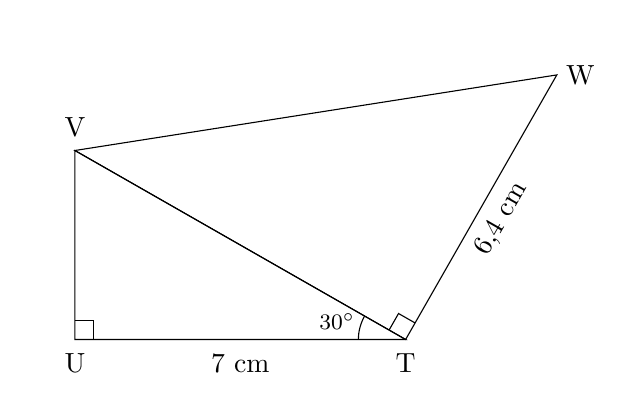
\begin{tikzpicture}[baseline,baseline=(current bounding box.north),scale = 0.6]

    \tikzset{
      point/.style={
        thick,
        draw,
        cross out,
        inner sep=0pt,
        minimum width=5pt,
        minimum height=5pt,
      },
    }
    \clip (-1,-1) rectangle (11.2,6.6000000000000005);
    	\draw[color={black}] (7,0)--(0,0)--(0,4)--cycle;
	\draw[color={black}] (0,4)--(7,0)--(10.2,5.6)--cycle;
	\draw[color={black}] (0.4,0)--(0.4,0.4)--(0,0.4);
	\draw[color={black}] (6.65,0.2)--(6.85,0.55)--(7.2,0.35);
	\draw [color={black}] (7,-0.5) node[anchor = center,scale=1, rotate = 0] {T};
	\draw [color={black}] (0,-0.5) node[anchor = center,scale=1, rotate = 0] {U};
	\draw [color={black}] (0,4.5) node[anchor = center,scale=1, rotate = 0] {V};
	\draw [color={black}] (10.7,5.6) node[anchor = center,scale=1, rotate = 0] {W};
	\draw (5.550234128106853,0.38494014689806405) node[anchor = center] {\footnotesize \color{black}{$30^\circ$}};
	\draw[color={black}] (6,0) arc (180:150.26:1) ;
	\draw [color={black}] (3.5,-0.5) node[anchor = center,scale=1, rotate = 0] {7 cm};
	\draw [color={black}] (9.03,2.55) node[anchor = center,scale=1, rotate = -299.74487999999997] {6,4 cm};

\end{tikzpicture}\\\\ \end{minipage}
	\item \begin{minipage}[t]{\linewidth} 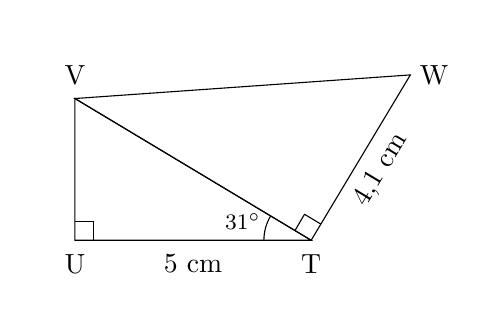
\begin{tikzpicture}[baseline,baseline=(current bounding box.north),scale = 0.6]

    \tikzset{
      point/.style={
        thick,
        draw,
        cross out,
        inner sep=0pt,
        minimum width=5pt,
        minimum height=5pt,
      },
    }
    \clip (-1,-1) rectangle (8.1,4.5);
    	\draw[color={black}] (5,0)--(0,0)--(0,3)--cycle;
	\draw[color={black}] (0,3)--(5,0)--(7.1,3.5)--cycle;
	\draw[color={black}] (0.4,0)--(0.4,0.4)--(0,0.4);
	\draw[color={black}] (4.66,0.21)--(4.86,0.55)--(5.21,0.34);
	\draw [color={black}] (5,-0.5) node[anchor = center,scale=1, rotate = 0] {T};
	\draw [color={black}] (0,-0.5) node[anchor = center,scale=1, rotate = 0] {U};
	\draw [color={black}] (0,3.5) node[anchor = center,scale=1, rotate = 0] {V};
	\draw [color={black}] (7.6,3.5) node[anchor = center,scale=1, rotate = 0] {W};
	\draw (3.5544144825649857,0.40035298398056335) node[anchor = center] {\footnotesize \color{black}{$31^\circ$}};
	\draw[color={black}] (4,0) arc (180:149.04:1) ;
	\draw [color={black}] (2.5,-0.5) node[anchor = center,scale=1, rotate = 0] {5 cm};
	\draw [color={black}] (6.48,1.49) node[anchor = center,scale=1, rotate = -300.96376] {4,1 cm};

\end{tikzpicture}\\\\ \end{minipage}
	\item \begin{minipage}[t]{\linewidth} 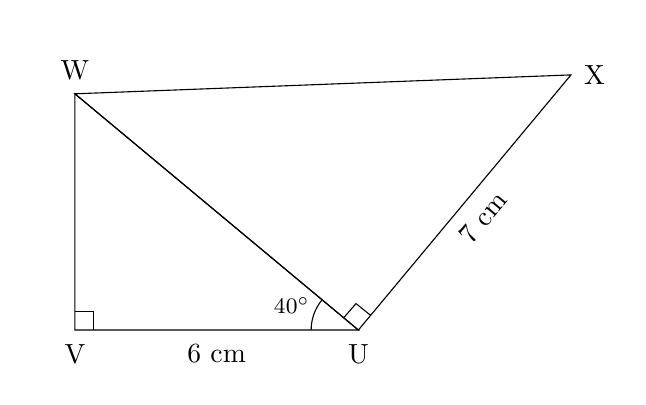
\begin{tikzpicture}[baseline,baseline=(current bounding box.north),scale = 0.6]

    \tikzset{
      point/.style={
        thick,
        draw,
        cross out,
        inner sep=0pt,
        minimum width=5pt,
        minimum height=5pt,
      },
    }
    \clip (-1,-1) rectangle (11.5,6.4);
    	\draw[color={black}] (6,0)--(0,0)--(0,5)--cycle;
	\draw[color={black}] (0,5)--(6,0)--(10.5,5.4)--cycle;
	\draw[color={black}] (0.4,0)--(0.4,0.4)--(0,0.4);
	\draw[color={black}] (5.69,0.26)--(5.95,0.56)--(6.26,0.31);
	\draw [color={black}] (6,-0.5) node[anchor = center,scale=1, rotate = 0] {U};
	\draw [color={black}] (0,-0.5) node[anchor = center,scale=1, rotate = 0] {V};
	\draw [color={black}] (0,5.5) node[anchor = center,scale=1, rotate = 0] {W};
	\draw [color={black}] (11,5.4) node[anchor = center,scale=1, rotate = 0] {X};
	\draw (4.589612370433775,0.5106924068033182) node[anchor = center] {\footnotesize \color{black}{$40^\circ$}};
	\draw[color={black}] (5,0) arc (180:140.19:1) ;
	\draw [color={black}] (3,-0.5) node[anchor = center,scale=1, rotate = 0] {6 cm};
	\draw [color={black}] (8.63,2.38) node[anchor = center,scale=1, rotate = -309.80557] {7 cm};

\end{tikzpicture}\\\\ \end{minipage}
\end{enumerate}

\end{exercice}

\end{document}
